\chapter{Introducción específica} % Main chapter title

\label{Chapter2}

%----------------------------------------------------------------------------------------
%	SECTION 1
%----------------------------------------------------------------------------------------
En este capítulo se presentan las tecnologías utilizadas e incorporadas en este trabajo. 

%Hacia el final se exponen los requerimientos que se deben cumplir %en el desarrollo.

\section{Servicios en la nube}
El cloud computing o servicios en la nube cobra cada vez más relevancia en las empresas debido, principalmente a la ventaja de no tener que hacer grandes inversiones en infraestructuras que mantengan aplicaciones, plataformas o servidores propios.

Los servicios en la nube se clasifican en:

\begin{itemize}
\item Infraestructura como Servicio (IaaS)
\item Plataforma como Servicio (PaaS)
\item \emph{software} como Servicio (SaaS)
\end{itemize}

En la figura \ref{fig:servicios}, se puede ver una representación gráfica para diferenciar las capas y su orientación para cada modelo de servicio.


\begin{figure}[htbp]
	\centering
	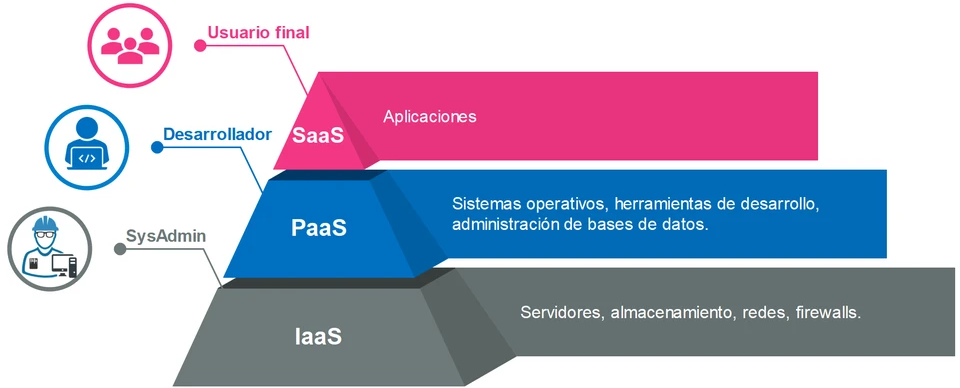
\includegraphics[width=.9\textwidth]{./Figures/servicios.png}
	\caption{Tipos de servicio y orientación por rol \protect\footnotemark.}

	\label{fig:servicios}
\end{figure}

\footnotetext{Imagen tomada de \url{https://openwebinars.net/blog/tipos-de-cloud-computing/}}

Para detallar el gráfico anterior, se describen los tipos de servicios de computación en la nube:

\vspace{1cm}

\begin{enumerate}

\item \keyword{IaaS}  (\emph{Infraestructure  as  a  Service})

Esta categoría ofrece servicios de infraestructura, entre ellos está la distribución de recursos de computación y almacenamiento cuyos precios varían conforme se realice el consumo. Es decir, se paga lo que se consume. Las empresas que los contratan nunca ven el equipo físico, pero sí pueden tener la experiencia del funcionamiento al momento de usar el servicio deseado \citep{BOOK:2}.

Ejemplo de IaaS:

\begin{itemize}
\item Amazon Web Services
\item Microsoft Azure
\item Google Cloud Platform
\end{itemize}

\vspace{0.5cm}

\item \keyword{PaaS} (\emph{Plataform as a Service}):

Este servicio ofrece plataformas de desarrollo sin necesidad de adquirir tecnología con costo muy elevado. El hardware y el \emph{software} en este modelo es administrado por el proveedor del servicio, además de que los desarrolladores no se preocupan por el rendimiento del hardware ni mucho menos por las actualizaciones del sistema operativo, ya que todo lo realiza el proveedor del servicio \citep{BOOK:2}.
 
Ejemplos de PaaS:

\begin{itemize}
\item AWS Elastic Beanstalk
\item Azure App Service
\item Google App Engine

\end{itemize}

\vspace{0.5cm}

\item \keyword{SaaS} (\emph{Software as a Service}): 

Constituye el modelo más utilizado porque, además de brindar servicio de \emph{software}, ofrece también el almacenamiento de la información que se genera desde el \emph{software}. Las ventajas notorias de este modelo son la simplicidad de integración, costo y escalabilidad. Se pueden indicar como desventajas la percepción de incidentes de seguridad y que la información se encuentra alojada en un espacio físico que no sea el de la propia empresa \citep{BOOK:2}. 

Ejemplos de SaaS:

\begin{itemize}
\item Microsoft Office 365
\item Aplicaciones web de Google
\end{itemize}

\vspace{0.5cm}

\end{enumerate}

En la figura \ref{fig:capas-servicios} se muestran las capas de cada servicio descrito y el acceso que el cliente tiene con cada modelo (capas de color verde).

\begin{figure}[htbp]
	\centering
	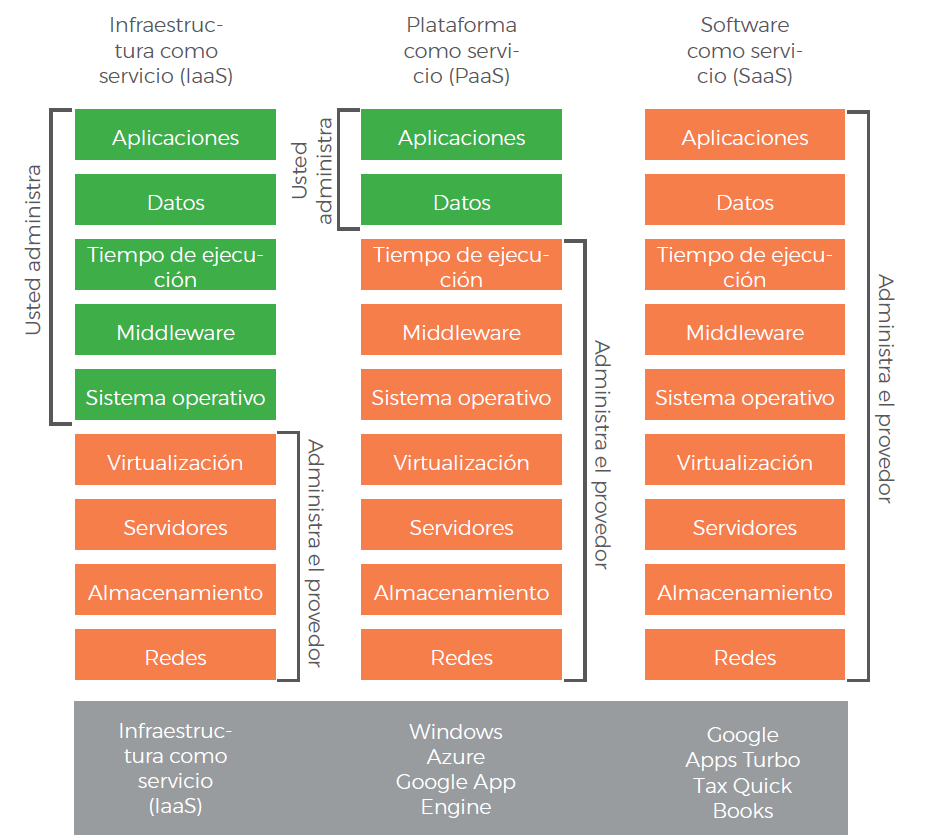
\includegraphics[width=.8\textwidth]{./Figures/capas-servicios.png}
	\caption{Infraestructura por capas según el tipo de servicio  \citep{BOOK:2}.}

	\label{fig:capas-servicios}
\end{figure}

%\footnotetext{Imagen tomada del libro \textit{Cloud Computing for Pymes}. \citep{BOOK:1}}}

Para el trabajo se usó el servicio tipo PaaS en la creación y configuración del \emph{broker} remoto y para almacenar la aplicación web así como para gestionar la base de datos.

\section{Protocolo MQTT}

\begin{itemize}
\item El broker MQTT

El servidor o broker es el programa que se encarga de recepcionar los mensajes enviados por los clientes y distribuirlos entre sí en un sistema publicador-suscriptor. Los clientes envían periódicamente paquetes y esperan la respuesta del broker, como se ilustra con la figura \ref{fig:broker}. 

\begin{figure}[htbp]
	\centering
	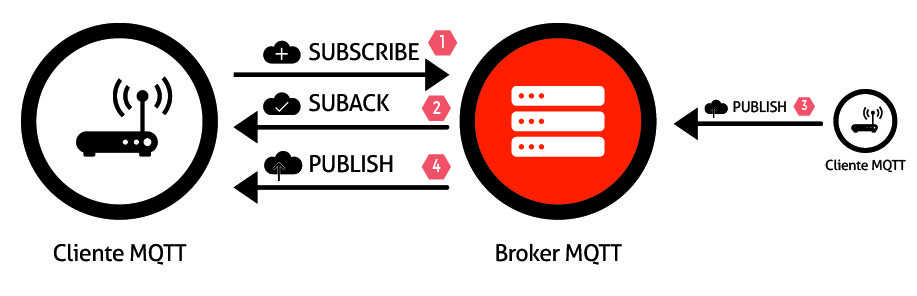
\includegraphics[width=.7\textwidth]{./Figures/broker.jpg}
	\caption{Funcionamiento del broker MQTT \protect\footnotemark.}

	\label{fig:broker}
\end{figure}

\footnotetext{Imagen tomada de \url{https://www.factor.mx/portal/base-de-conocimiento/mqtt/}}

La comunicación puede estar cifrada mediante TLS (\emph{Transport Layer Security}) y contar con credenciales de acceso para el control de los canales de envío y recepción. Al broker se le puede conectar un sin fin de dispositivos como teléfonos móviles, computadoras, sensores, actuadores, lámparas, relojes, bombas de agua e, incluso, refrigeradores, cocinas y mucho más. 

%\vspace{1cm}
\vspace{1cm}
\item El protocolo MQTT

MQTT (\textit{Message Queue Telemetry Transport}) es un protocolo de red ligero de publicación-suscripción que transporta mensajes entre dispositivos. El protocolo generalmente se ejecuta sobre TCP / IP ; sin embargo, cualquier protocolo de red que proporcione conexiones bidireccionales ordenadas y sin pérdidas puede admitir MQTT. Está diseñado para conexiones con ubicaciones remotas donde existen restricciones de recursos o el ancho de banda de la red es limitado \citep{WEBSITE:3}. Su modelo de comunicación lo podemos ver en la figura \ref{fig:mqtt}.

\vspace{0.5cm}

\begin{figure}[htbp]
	\centering
	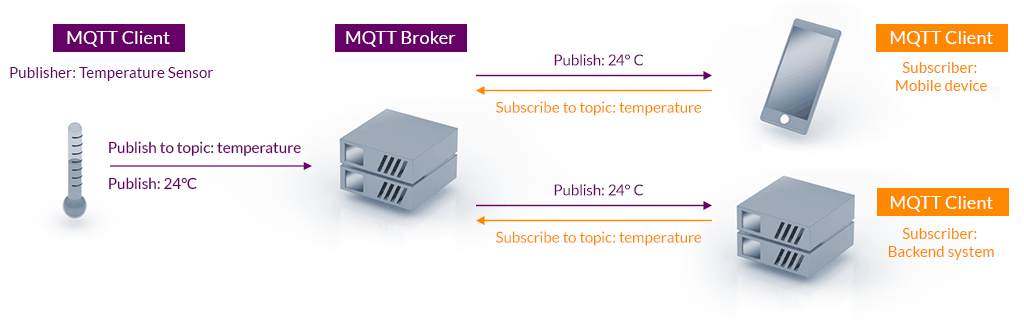
\includegraphics[width=.9\textwidth]{./Figures/mqtt.png}
	\caption{Ejemplo de funcionamiento del protocolo MQTT \protect\footnotemark.}
	\label{fig:mqtt}
\end{figure}

\footnotetext{Imagen tomada de \url{https://mqtt.org/}}


MQTT es un protocolo de mensajería estándar para IoT. Está diseñado como un transporte de mensajería de extremadamente liviano y se utiliza en una amplia variedad de industrias, como la automotriz, la fabricación, las telecomunicaciones, el petróleo y el gas, etc \citep{WEBSITE:4}. 
\end{itemize}

\section{Elementos del broker MQTT}

Antes de construir una red MQTT, es necesario entender los conceptos que se utiliza para crear una red para IoT: 
\begin{itemize}
\item Cliente: un dispositivo que puede publicar mensajes, suscribirse para recibir mensajes, o ambos.
\item Broker: es el servidor que acepta mensajes publicados por clientes y los difunde entre los clientes suscritos.
\item Publicar: cuando un cliente envía un mensaje al broker usando un tópico.
\item Tópico: los mensajes deben estar etiquetados con algún tópico o tema. Los clientes se suscriben a tópicos específicos, de manera que solo reciben los mensajes publicados con dichos tópicos. 
\end{itemize}

El broker MQTT usado en el proyecto es Eclipse Mosquitto, por ser de código abierto.

\section{Eclipse Mosquitto} 
Eclipse Mosquitto es un agente de mensajes de código abierto (con licencia EPL / EDL) que implementa las versiones 5.0, 3.1.1 y 3.1 del protocolo MQTT. Mosquitto es liviano y adecuado para su uso en todos los dispositivos, desde computadoras de placa única de baja potencia hasta servidores completos \citep{WEBSITE:5}.

El protocolo MQTT proporciona un método ligero para realizar mensajes mediante un modelo de publicación / suscripción. Esto lo hace adecuado para la mensajería de Internet de las cosas, como con sensores de baja potencia o dispositivos móviles como teléfonos, computadoras integradas o microcontroladores \citep{WEBSITE:5}.

Mosquitto es parte de la Fundación Eclipse, es un proyecto de \url{iot.eclipse.org} y está patrocinado por \url{cedalo.com} \citep{WEBSITE:5}. 

\section{Hardware del servidor local} 

El hardware del módulo principal integra la placa raspberry Pi 4 modelo B de 8 GB como placa base. La Raspberry Pi es una serie de ordenadores de placa reducida, ordenadores de placa única u ordenadores de placa simple (SBC) de bajo costo desarrollado en el Reino Unido por la Raspberry Pi Foundation, con el objetivo de poner en manos de las personas de todo el mundo el poder de la informática y la creación digital \citep{WEBSITE:6}.

La placa Raspberry Pi 4 es una pequeña computadora de escritorio de doble pantalla con opciones de salida en 4K, se puede usar para cerebros de robot, centros de hogar inteligente, centros de medios, núcleos de IA (inteligencia artificial) en red, controladores de fábrica y mucho más. La figura \ref{fig:rpi4} muestra sus principales especificaciones.

\vspace{0.5cm}

\begin{figure}[htbp]
	\centering
	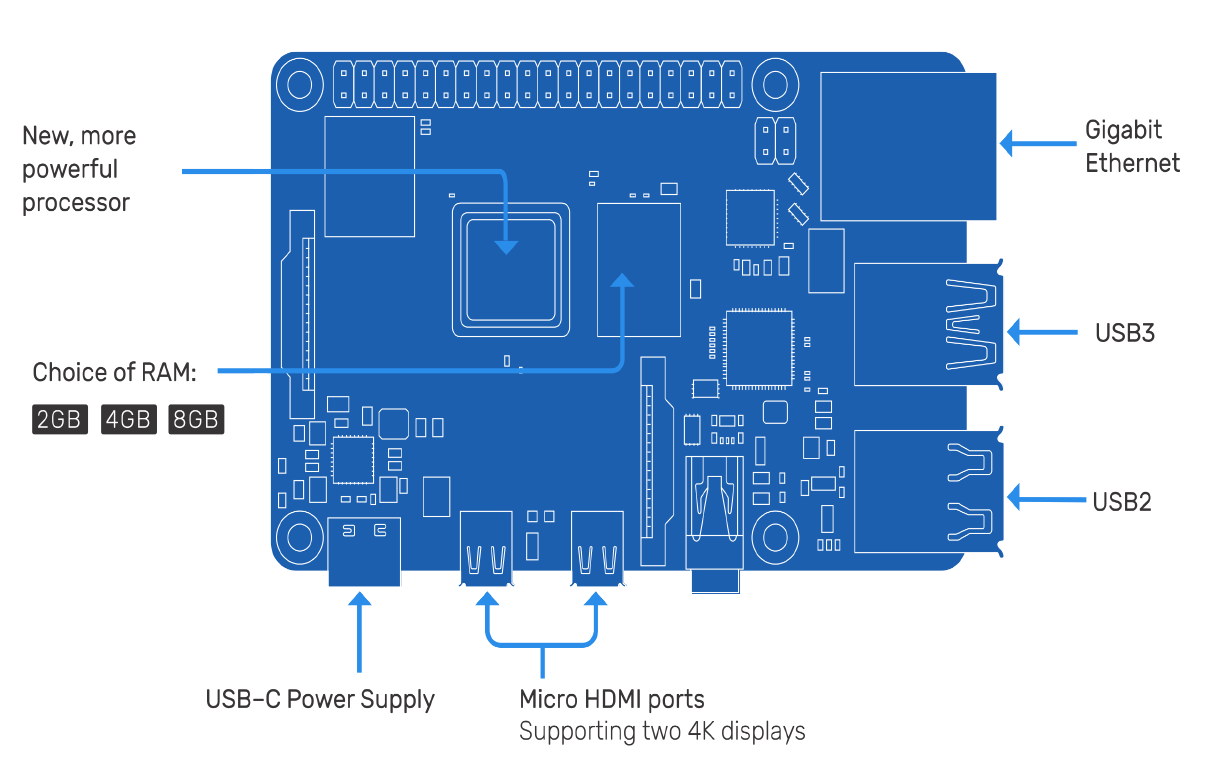
\includegraphics[width=1.0\textwidth]{./Figures/rpi4.png}
	\caption{Computadora Raspberry Pi 4 \protect\footnotemark. \citep{WEBSITE:7}}

	\label{fig:rpi4}
\end{figure}

\footnotetext{Imagen de \url{https://www.raspberrypi.com/products/raspberry-pi-4-model-b/specifications/}}

\vspace{1cm}

Especificaciones técnicas de la computadora Raspberry Pi 4 \citep{WEBSITE:7}:

\begin{itemize}
\item Broadcom BCM2711, SoC de 64 bits Cortex-A72 de cuatro núcleos (ARM V8) a 1,5 GHz
\item SDRAM LPDDR4-3200 de 2 GB, 4 GB u 8 GB (según el modelo)
\item 2.4 GHz y 5.0 GHz IEEE 802.11ac inalámbrica, Bluetooth 5.0, BLE
\item Gigabit Ethernet
\item Puertos USB 3.0; 2 puertos USB 2.0.
\item Cabecera GPIO estándar Raspberry Pi de 40 pines (totalmente compatible con las placas anteriores)
\item Puertos micro-HDMI (hasta 4kp60 compatible)
\item Puerto de pantalla MIPI DSI de 2 carriles
\item Puerto de cámara MIPI CSI de 2 carriles
\item Puerto de video compuesto y audio estéreo de 4 polos
\item H.265 (decodificación 4kp60), H264 (decodificación 1080p 60, codificación 1080p 30)
\item Ranura para tarjeta microSD para cargar el sistema operativo y el almacenamiento de datos
\item 5 VCC a través del conector USB-C (mínimo 3 A)
\item 5 VCC a través del encabezado GPIO (mínimo 3 A)
\item Power over Ethernet (PoE) habilitado (requiere PoE HAT separado)
\item Temperatura de funcionamiento: 0 - 50 C° ambiente
\end{itemize}

\subsection{Sistema operativo para el servidor local}

En la actualidad existen mucha variedad de sistemas operativos para la placa Raspberry Pi, pero para este proyecto se uso el sistema operativo oficial y recomendado por la Raspberry Pi Foundation, llamado ``Raspberry Pi OS''.

La web oficial ofrece diversas versiones a las cuales se puede acceder con descarga directa como se ilustra con la figura \ref{fig:so}.

\begin{figure}[htbp]
	\centering
	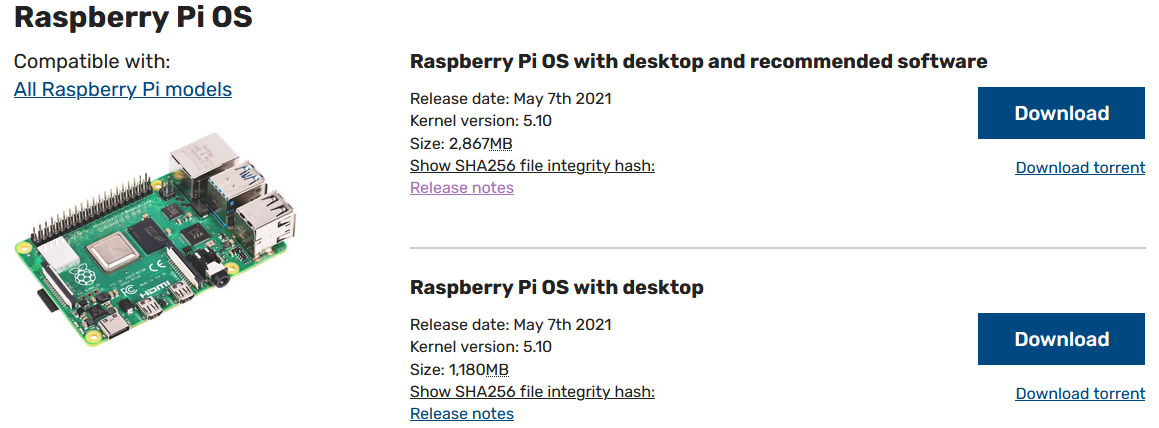
\includegraphics[width=.95\textwidth]{./Figures/so.png}
	\caption{Versiones del sistema operativo para Raspberry Pi \protect\footnotemark.}
	\label{fig:so}
\end{figure}

\footnotetext{Imagen tomada de \url{https://www.raspberrypi.com/software/operating-systems/}}

\section{Hardware y software utilizado para los módulos}

Los componentes principales usados en el desarrollo de cada módulo están formados por una placa base NodeMCU, sensores y actuadores.

\subsection{Placa NodeMCU ESP8266}

La tarjeta NodeMCU es de bajo costo y está basado en el procesador ESP8266, un procesador que está utilizándose mucho para la realización de proyectos IoT, ya que dispone de Wi-Fi integrado. El procesador se programa en Lua, pero también se puede programar con Arduino IDE. Su principal diferencia es que este procesador trabaja a 3.3V.  Además, ofrece más ventajas como la incorporación de un regulador de tensión integrado, así como un puerto USB de programación. 

En el mercado actual se encuentran dos versiones muy utilizadas de la familia NodeMCU y la forma rápida de diferenciar la V2 de la V3, es fijarnos en el conversor serial que monta y en su tamaño. El CP2102 (V2) que es cuadrado, y el CH340G (V3) que es más alargado respectivamente, como se ilustra con la figura \ref{fig:nodemcu}.
 

\begin{figure}[htbp]
	\centering
	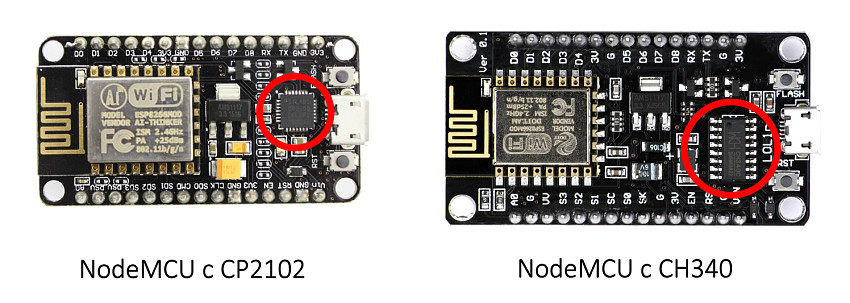
\includegraphics[width=.85\textwidth]{./Figures/NodeMcu.jpg}
	\caption{Diferencia visual entre los modelos NodeMCU.}

	\label{fig:nodemcu}
\end{figure}

Para el trabajo se usó la versión 3 del NodeMCU ESP8266.

Especificaciones técnicas del NodeMCU:

\begin{itemize}
\item Utiliza chip CH340G (USB).
\item Tensión de alimentación: 4.5 V~9 V (10 V max) y/o alimentación por USB.
\item Tensión de pines I/O: 3.3 V.
\item Wireless 802.11 b/g/n standard
\item Wi-Fi at 2.4 GHz, soporta encriptación WPA/WPA2
\item Soporta tres modos de operación: STA/AP/STA+AP
\item Pila de almacenamiento para protocolo TCP/IP (5 conexiones máximo)
\item Pines: D0~D8, SD1~SD3 pueden ser usados como GPIO, PWM, IIC con capacidad de drenar 15 mA por pin.
\item 1 canal ADC: AD0
\item Consumo de corriente continua ≈ 70 mA (200 mA MAX), Standby: <200 uA
\item Velocidad de transmisión: 110 - 460800 bps
\item Soporta interfaz de comunicación UART/GPIO
\item OTA: Remote firmware upgrade
\item Soporta Smart Link Smart Networking
\item Temperatura de trabajo: -40 ℃ ~ +125 ℃
\item Memoria: 4 MByte
\end{itemize}

\subsection{Sensor de temperatura y humedad DHT11}

El DHT11 es un sensor de humedad relativa y temperatura de media precisión a un bajo precio. La salida suministrada es de tipo digital utilizando solamente un pin de datos (no posee salida analógica). Es utilizado en aplicaciones académicas relacionadas al control automático de temperatura, aire acondicionado, monitoreo ambiental en agricultura y más. El sensor se muestra en la figura \ref{fig:dht11}.

Utilizar el sensor DHT11 con las plataformas Arduino, Raspberry Pi y Nodemcu es muy sencillo tanto a nivel de \emph{software} como hardware. A nivel de \emph{software} se dispone de librerías para Arduino con soporte para el protocolo \emph{Single bus}. En cuanto al hardware, solo es necesario conectar el pin VCC de alimentación a 3 V - 5 V, el pin GND a Tierra y el pin de datos a un pin digital de Arduino \citep{WEBSITE:8}. 

\begin{figure}[htbp]
	\centering
	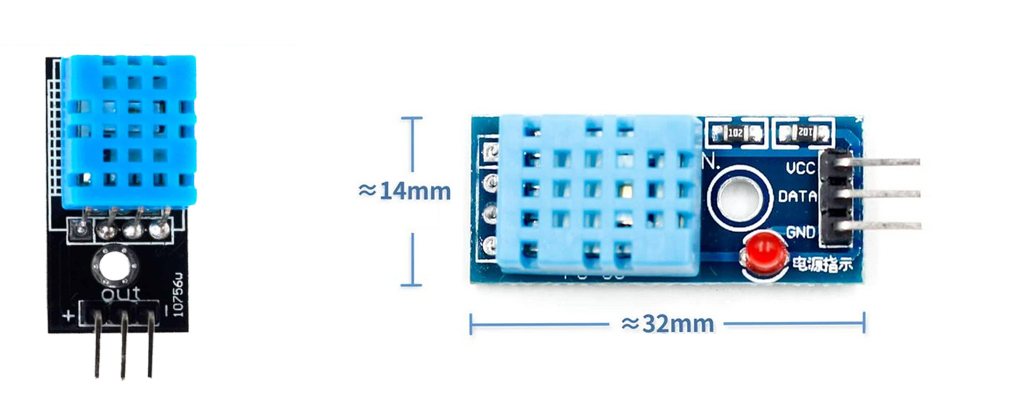
\includegraphics[width=.8\textwidth]{./Figures/dht11.jpg}
	\caption{Modelo y dimensiones del sensor DHT11. }

	\label{fig:dht11}
\end{figure}

Especificaciones técnicas del sensor:

\begin{itemize}
\item Tensión de Operación: 3 V - 5 V DC
\item Rango de medición de temperatura: 0 a 50 °C
\item Precisión de medición de temperatura: ±2.0 °C
\item Resolución Temperatura: 0.1°C
\item Rango de medición de humedad: 20\% a 90\% RH.
\item Precisión de medición de humedad: 5\% RH.
\item Resolución Humedad: 1\% RH
\item Tiempo de sensado: 1 seg.
\item Interface digital: Single-bus.
\item Modelo: DHT11
\item Peso: 1 gr.
\item Carcasa de plástico celeste
\end{itemize}

\subsection{Sensor de Corriente AC SCT-013-030}

La familia SCT-013 son sensores de corrientes no invasivos que permiten medir la intensidad que atraviesa un conductor sin necesidad de cortar o modificar el conductor. Podemos emplear estos sensores con un procesador como Arduino para medir la intensidad o potencia consumida por una carga. Los sensores SCT-013 son transformadores de corriente, dispositivos de instrumentación que hacen posible una medición proporcional a la intensidad que atraviesa un circuito. La medición se realiza por inducción electromagnética \citep{WEBSITE:9}. 

Los sensores SCT-013 disponen de un núcleo ferromagnético partido (como una pinza) que permite abrirlo para arrollar un conductor de una instalación eléctrica sin necesidad de cortarlo, como se ilustra con la figura \ref{fig:sensorCorriente}. Dentro de la familia SCT-013 existen modelos que proporcionan la medición como una salida de intensidad o de tensión. Se recomienda usar sensores de salida por tensión porque la conexión es más sencilla \citep{WEBSITE:9}. 

\begin{figure}[htbp]
	\centering
	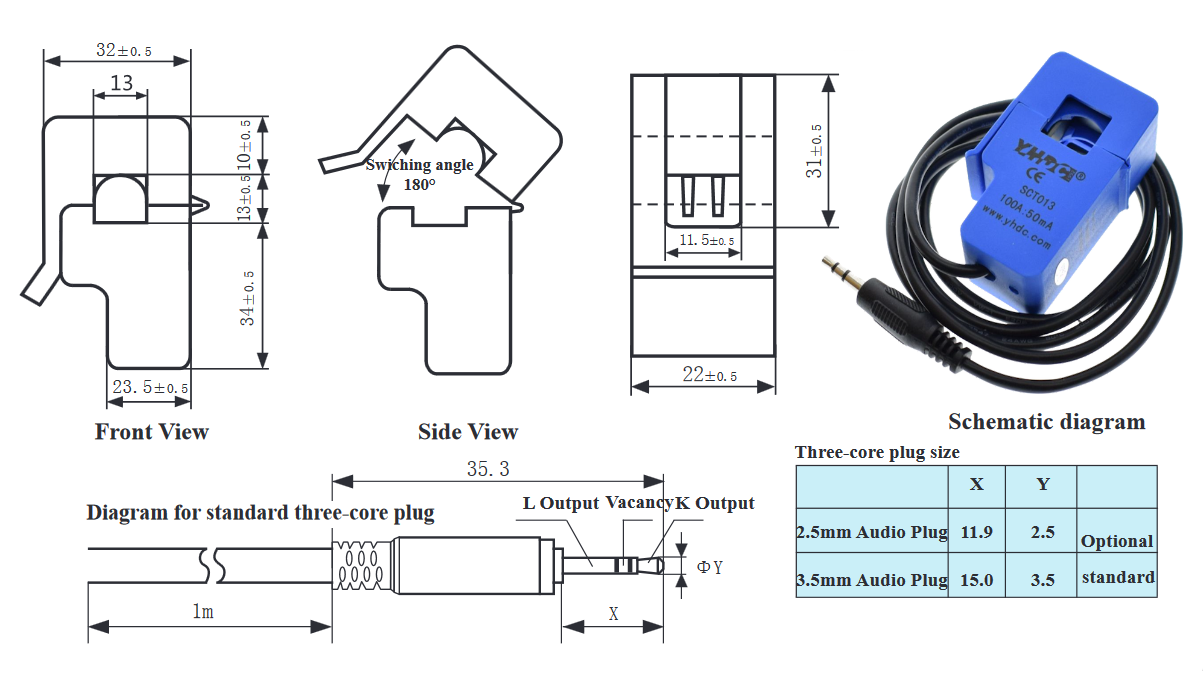
\includegraphics[width=1.0\textwidth]{./Figures/sensorCorriente2.png}
	\caption{Modelo y dimensiones del sensor SCT-013-030 AC \protect\footnotemark.}

	\label{fig:sensorCorriente}
\end{figure}

\footnotetext{Imagen de \url{https://datasheetspdf.com/pdf-file/1004704/XiDiTechnology/SCT-013-030/1}}

El sensor SCT-013 es muy fácil de manejar y acoplar. Puede colocarse como una pinza alrededor de un cable que entre al edificio sin la necesidad de realizar algún trabajo de alta tensión, adecuado para la medición de corriente AC, monitoreo y protección de motores AC, equipo de iluminación, etc \citep{WEBSITE:10}.

Especificaciones técnicas del sensor de corriente:

\begin{itemize}
\item Corriente de entrada (inducción): 0-30 A AC
\item Modo de salida: 0 - 1 V
\item No linealidad: ±1%
\item Resistencia (RL): 62 $\Omega $
\item Grado de Resistencia: Grade B
\item Temperatura de operación: -25 °C ~ ﹢70 °C
\item Longitud del cable: 1m
\item Tamaño abierto: 13 mm x 13 mm
\end{itemize}

Para el trabajo se consideró el módulo SCT-013 de 30 A y con soporte para 250 VAC.

\subsection{Relé Actuador}

Un relé es un interruptor que podemos activar mediante una señal eléctrica. En su versión más simple es un pequeño electro-imán que cuando lo excitamos mueve la posición de un contacto eléctrico de conectado a desconectado o viceversa. Un relé es un interruptor, que utiliza una pequeña corriente para accionar un circuito mayor. Se aplica una señal en la entrada que enciende otro circuito conectado en la salida, sin necesidad de supervisión humana.

Los relés más utilizados son módulos que son capaces de activarse mediante la entrada de 5 V. La capacidad de elegir el módulo relé adecuado para nuestro trabajo dependerá de la tensión y amperaje que debe gestionar el relé. En la figura \ref{fig:rele} se aprecian dos modelos de módulos relé con capacidad de activación 5 V y con soporte para 10 A - 250 VAC y 30 A – 250 VAC respectivamente.


\begin{figure}[htbp]
	\centering
	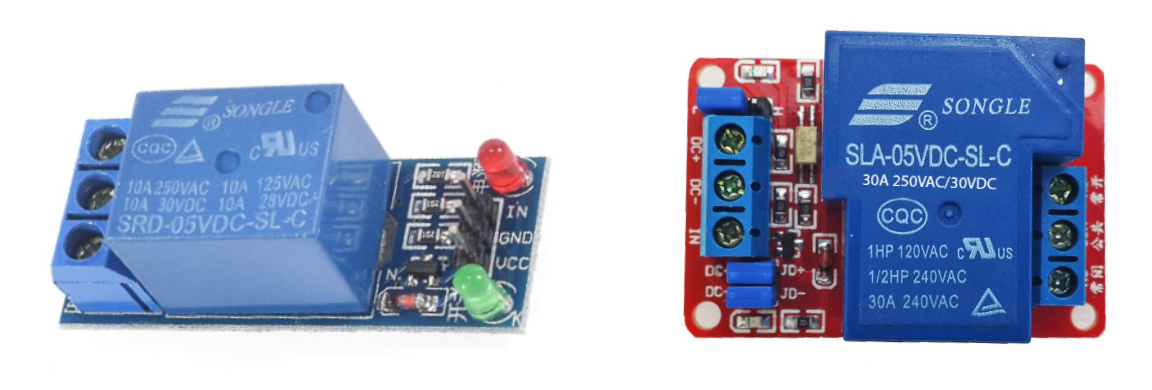
\includegraphics[width=1.0\textwidth]{./Figures/rele.jpg}
	\caption{Modelos de relés con activación de 5 V.}

	\label{fig:rele}
\end{figure}

El relé es un interruptor nos permite trabajar con dos circuitos, uno con tensiones elevadas, por ejemplo, 220 V pero que es activado por un circuito de tensión inferior, por ejemplo, 5 V.

Para el trabajo se consideró el módulo relé de activación 5 V y con soporte para 30 A - 250 VAC.

\subsection{Lenguajes de programación}

La elaboración de este trabajo involucró el usó de distintos \emph{software}s como herramientas para facilitar el desarrollo, así como el uso de diversos lenguajes de programación que se describen a continuación:
\begin{itemize}
\item Python: es un lenguaje de programación interpretado cuya filosofía hace hincapié en la legibilidad de su código. Se trata de un lenguaje de programación multiparadigma, ya que soporta parcialmente la orientación a objetos, programación imperativa y, en menor medida, programación funcional.

Se utilizó para la creación de procesos internos en el módulo principal. 
\item PHP: es un lenguaje de programación de usó general que se adapta especialmente al desarrollo web del lado \emph{backend}.

Se utilizó como lenguaje \emph{backend} del \emph{software} de monitoreo y control.
\item JavaScript: lenguaje de programación interpretado utilizado en el lado del cliente, es el único lenguaje de programación que funciona en los navegadores de forma nativa (lenguaje interpretado sin necesidad de compilación).

Se utilizó como lenguaje frontend del \emph{software} de monitoreo y control.
\item Arduino: lenguaje de programación que está basado en C++.

Se utilizó como lenguaje para programar el firmware de los módulos de sensores y actuadores.
\end{itemize}